%
\documentclass[12pt]{article}

%% make references and citations clickable
\usepackage[backref,colorlinks=true, linkcolor=blue, citecolor=blue, urlcolor=blue, pdfborder={0 0 0}]{hyperref}

%% set the paper geometry
\usepackage[left=1in,top=1in,right=1in,bottom=1in,letterpaper]{geometry}

%% this is for arrows with text over them  --- currently not installed
%%\usepackage{mathtools}

%% uncomment the next line if you need to present an algorithm
%\usepackage{algorithm,algorithmic}

% This section is added by me (Geoff)
%-----------------------------------------------
%% standard AMS stuff
\usepackage{amssymb,amsmath,amsthm}

%% some proof-writing environments
\newenvironment{claim}[1]{\par\noindent\underline{Claim:}\space#1}{}
\newenvironment{claimproof}[1]{\par\noindent\underline{Proof:}\space#1}{}
%\newenvironment{proof}{\paragraph{Proof:}}{\hfill}
\theoremstyle{definition}
\newtheorem{theorem}{Theorem}[section]
\newtheorem{ex}[theorem]{Example}
\newtheorem{defn}[theorem]{Definition}
\newtheorem{lemma}[theorem]{Lemma}
\newtheorem{notn}[theorem]{Notation}

%% norm and abs val and inner prod
\newcommand{\norm}[1]{\left\lVert#1\right\rVert}
\newcommand{\abs}[1]{\left\lvert#1\right\rvert}
\newcommand{\iprod}[1]{\langle #1 \rangle}
\newcommand{\spn}[0]{\text{span}}

%% ceiling and floor   --- Not working for some reason
%%\DeclarePairedDelimiter\ceil{\lceil}{\rceil}
%%\DeclarePairedDelimiter\floor{\lfloor}{\rfloor}

%% kernel and image  -- Currently did something wrong
%%\newcommand{\ker}[1]{\text{ker}\left(#1\right)}
%%\newcommand{\Im}[1]{\text{Im}\left(#1\right)}  %% TODO: FIX THIS

%% Important letters/symbols
\newcommand{\ep}[0]{\epsilon}
\newcommand{\R}[0]{\mathbb{R}}
\newcommand{\bR}[0]{\bar{\mathbb{R}}}
\newcommand{\cC}[0]{\mathcal{C}}
\newcommand{\cP}[0]{\mathcal{P}}
\newcommand{\pd}[0]{\partial}

%% I had some issues with alignment, here was one online soln
%%\usepackage[fleqn]{amsmath}
%% It DIDN'T WORK THOUGH

%------------------------------------------------


%% for including urls by \url{url text}
\usepackage{url}

\usepackage{graphicx}

\begin{document}

\title{Meeting Notes 12-6-2016: Optical-Lidar Classification}
\author{Geoffrey Iyer}
\maketitle

The purpose of this file is to show some of our early classification results on the Optical/Lidar datasets. A quick recap: we use eigenvectors of the Graph-Laplacian to get an approximate solution to the graph min-cut problem. Let $X = \{x_1,x_2,\ldots,x_n\}$ represent te first dataset, and $Y = \{y_1,y_2,\ldots,y_n\}$ represent the second. We assume that the points are co-registered, i.e. that $x_j$ corresponds to $y_j$ in some natural physical way (in our examples, these are the same pixels captured with different cameras). Then define the graph $G$ with $n$ vertices (representing our $n$ data points) and edge weights defined by
\[w_{ij} = \max\left(\norm{x_i - x_j}_X , \norm{y_i-y_j}_Y\right).\]
Here we assume that $\norm{\cdot}_X$ and $\norm{\cdot}_Y$ are scaled such that they are comparable.

After defining the graph, we construct the Graph Laplacian and find eigenvectors (using the Nystrom Extension to keep computation time reasonable), then apply kmeans to the eigenvectors to get the final classifcation shown below.

Instead of using the maximum (i.e. the $L^\infty$ norm) I've also tried using an $L^p$ norm for many different values of $p$. There is rarely much of a difference in the end result.

\begin{figure}
  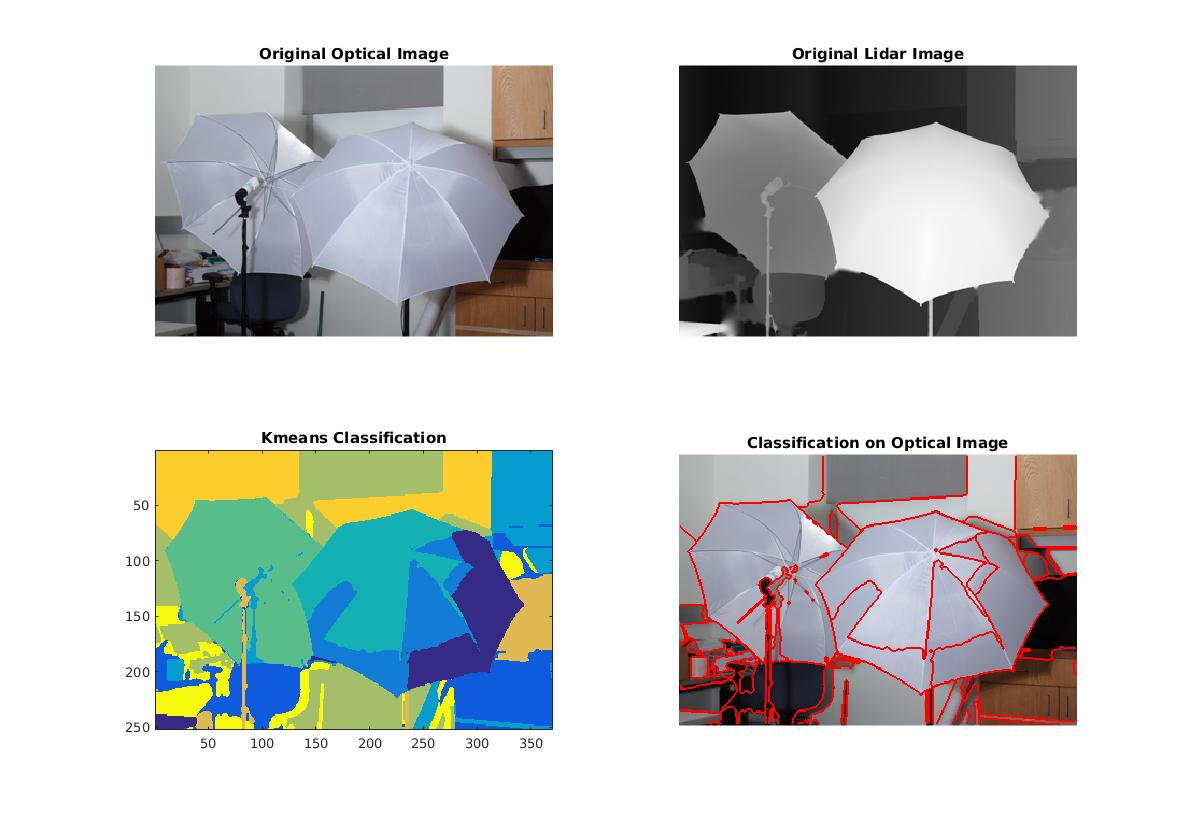
\includegraphics[width = \textwidth]{Umbrella.jpg}
  \caption{Classification on Umbrella Dataset}
\end{figure}

\begin{figure}
  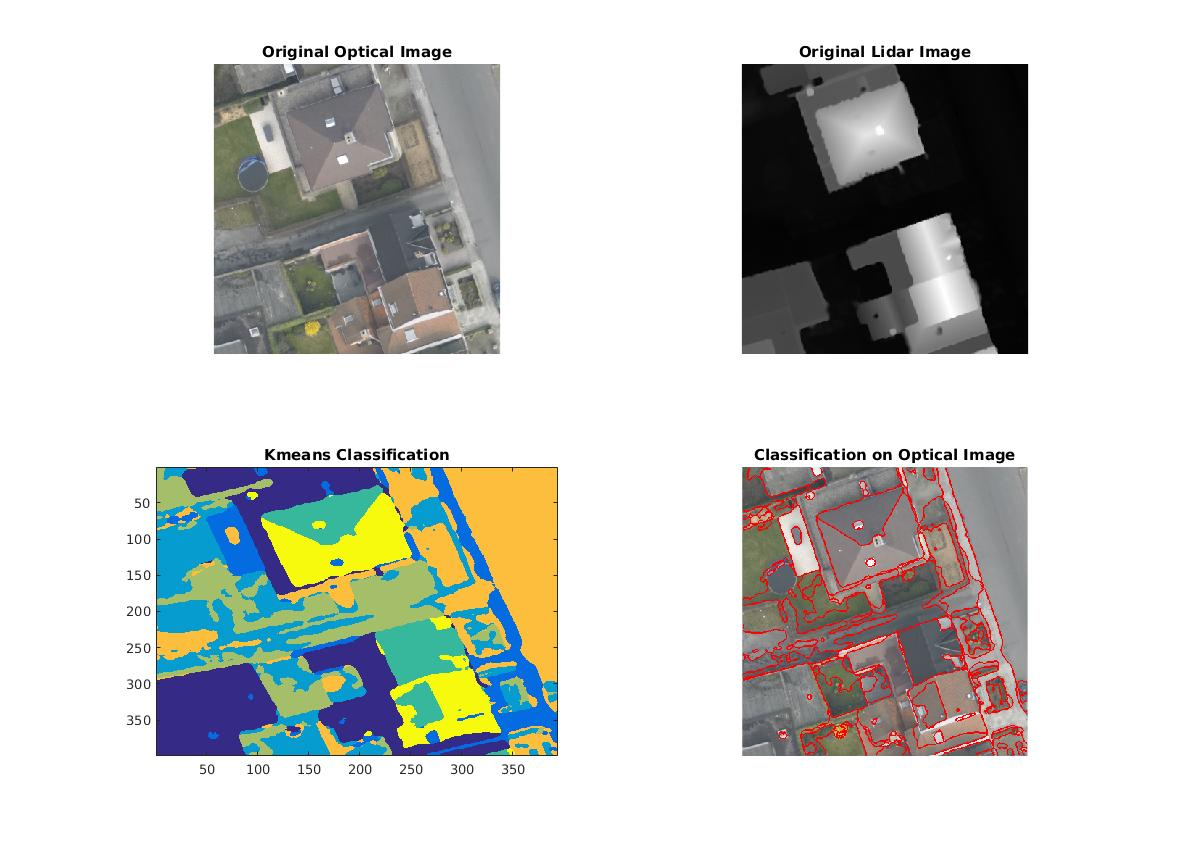
\includegraphics[width = \textwidth]{House(DFC2015).jpg}
  \caption{Classification on Houses Dataset (DFC2015)}
\end{figure}

\begin{figure}
  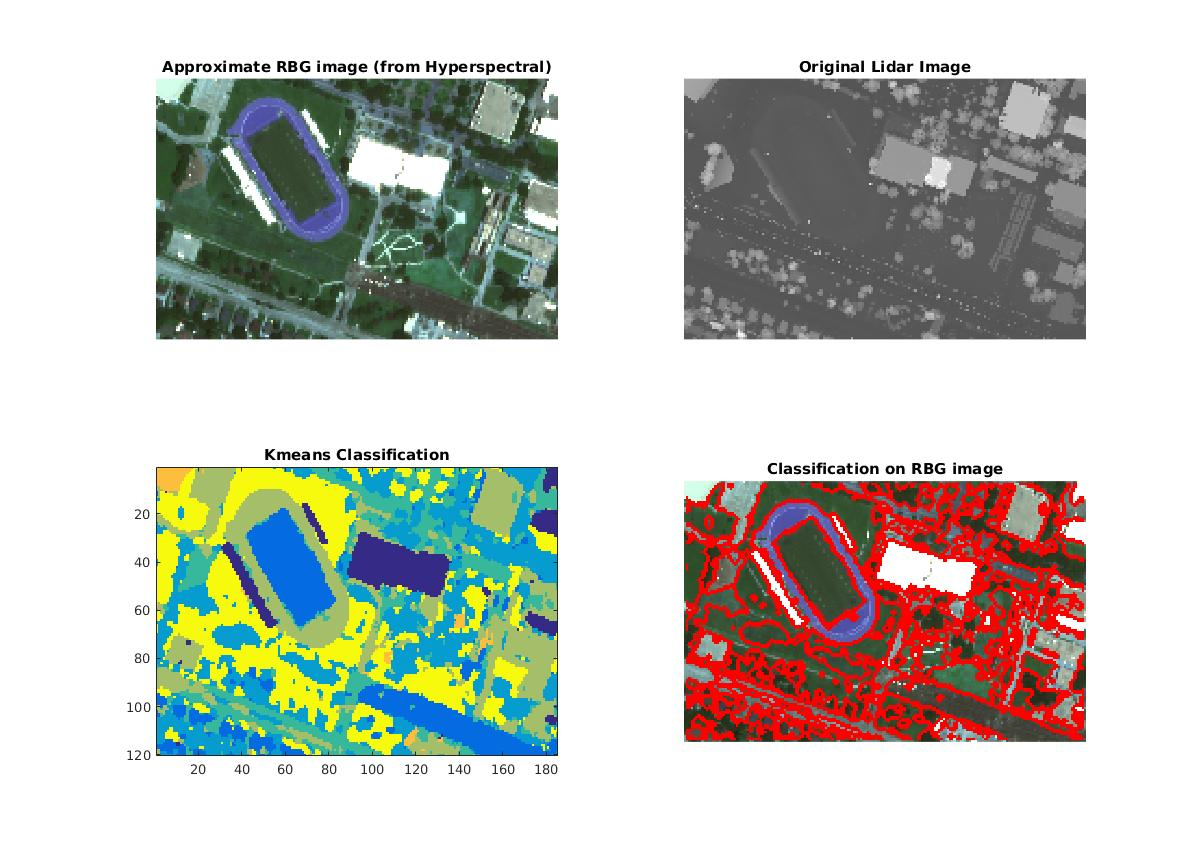
\includegraphics[width = \textwidth]{Stadium(DFC2013).jpg}
  \caption{Classification on Stadium Dataset (DFC2013)}
\end{figure}

\end{document}